\section{Architecture Technique}
L'amélioration du système d’information de l'entreprise passe tout d'abord
par une augmentation du nombre de postes informatiques. Toutes les
informations passeront par le système informatique et seront enregistrées.

\subsection{Schéma}

\begin{figure}[!h]
\begin{center}
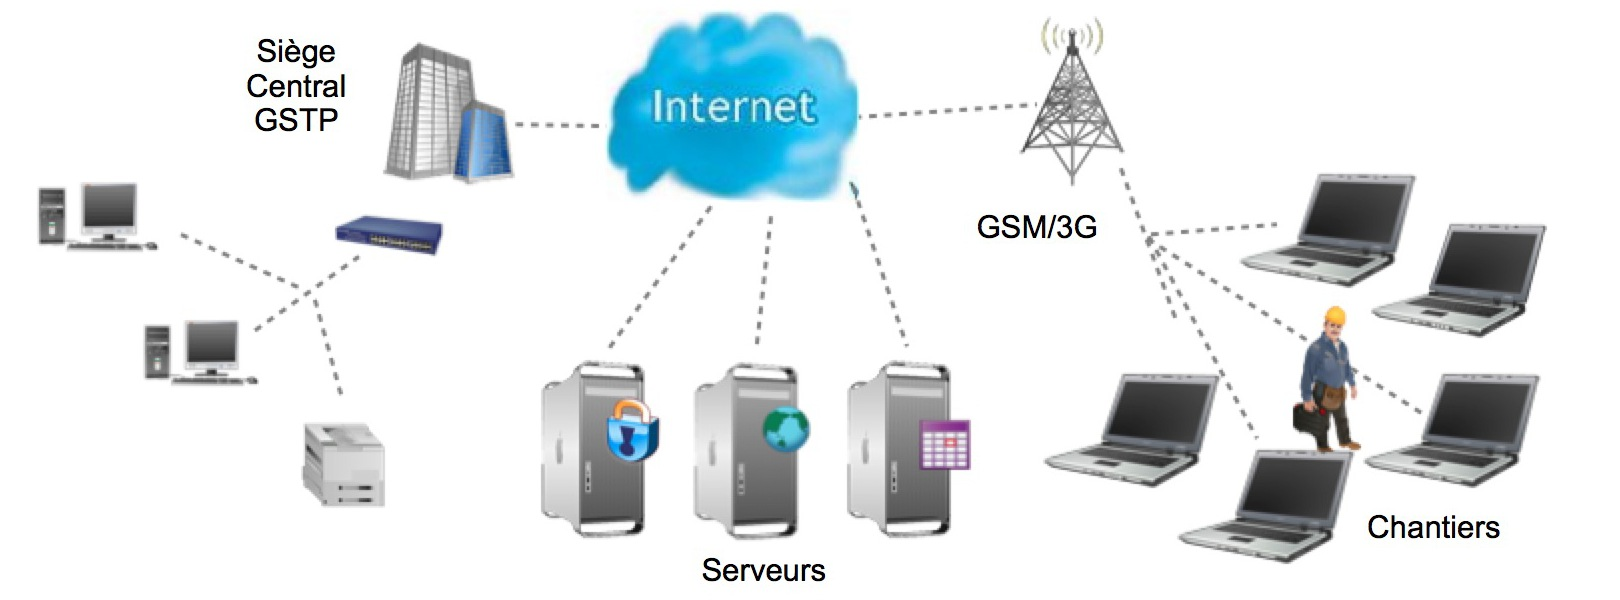
\includegraphics[width=13cm]{\PIXPATH/architech}
\caption{Schéma de l'organisation globale du SI}
\end{center}
\end{figure}


\subsection{Serveur}

Le serveur sera externalisé et servira de support pour la base de
données et la gestion des accès à ces données. 

Chaque application, et donc chaque poste, sera configurée pour se connecter
à la base de données du serveur.  Toutes partageront les mêmes informations
et il sera ainsi possible de facilement faire le rapprochement entre les
achats et le matériel réceptionné par exemple.

	\subsubsection{Architecture}
Nous avons besoin d'un serveur d'application qui hébergera les applications
pour le chantier, le magasin, et les différents départements,  ainsi qu'une
base de données pour les information concernant aux chantiers, magasin,
fournisseurs, etc. 

Pour établir la communication client-serveur on utilisera le protocole
LDAP. Il fournit à l'utilisateur des commandes pour se connecter ou se
déconnecter,  pour rechercher, comparer, créer, modifier ou effacer des
entrées.  Des mécanismes de chiffrement (SSL ou TLS) et d'authentification
(SASL), couplés à des mécanismes de règles d'accès (ACL) permettent de
protéger les transactions et l'accès aux données.

	\subsubsection{Hébergement}
    Il nous faut un ensemble de serveurs capables de répondre à un grand
    nombre de requêtes, et ce en permanence.

Une solution consiste à héberger nos serveurs dans le \textsl{cloud}, on
utilisera le modèle IAAS pour  que l'entreprise maintient ses applications,
les {\sl runtimes}, l'intégration SOA, les bases de données, le logiciel
serveur.  Cette solution nous permettant ainsi de payer uniquement les
ressources que nous consommons, tout en bénéficiant d'une bonne résilience
aux pannes et d'une bonne disponibilité.  L'entreprise GoGrid fournit un
tel service, à partir de 60 \euro par mois.


\subsection{Communication}
Le département Achat, Matériel et Maintenance doivent être en réseau local
pour qu'ils puissent  communiquer entre elles.

Sur les chantiers, il faut pouvoir relier les ordinateurs au siège par
l'intermédiaire d'Internet.  Nous savons que les chefs de chantiers sont
souvent amenés à se déplacer dans le cadre de leur travail, donc le réseau
3G est indispensable pour qu'ils puissent être plus réactif vis-à-vis de
leur activité, comme par exemple, répondre instantanément à un email,
rechercher une information, ou échanger et communiquer sur une messagerie. 

Chaque poste disposera d’une clé 3G pour se connecter au réseau GSM haut
débit.

Il existe une large choix de formules proposées par les différents
opérateurs de téléphones portables, nous prendrons une offre illimitée pour un prix 
d'environ 30 \euro par mois.

\subsection{Chantiers}

Nous renouvellerons l'ensemble de la flotte des PC utilisés de manière nomade.
Ces PC auront des caractéristiques correspondant au milieu de
travail (des ordinateurs résistantes à la pression, aux vibration, à
l'humidité, etc.  en fournissant un poste par chantier), ces ordinateurs
n'ont pas besoin d’être très performants, car ils ne servent qu'à se
connecter à Internet et faire fonctionner l'application de chantier.

\paragraph{Exemple : DELL ATG D620}\hfill\\
Ce PC portable résiste à l'humidité, l'altitude,
la pression, les vibrations, protégé contre les coups.
Ses caractéristiques techniques sont limitées mais largement suffisantes
(Core 2 Duo, 4Go de RAM, disque dur de 80Go) ; le prix : 499 \euro.
